\chapter{Reconstrucci\'{o}n tridimensional}
\label{chap:reconstruccion}
\epigraph{Going from the written, flat word to the three-dimensional object, that was one of the more enriching things that I've done.}{James Sanborn}

%@TODO que no se hizo/alcances/hipotesis
En este cap\'{i}tulo se describe c\'{o}mo utilizar la informaci\'{o}n obtenida hasta el momento para reconstruir tridimensionalmente el objeto. Las matrices de la c\'{a}mara (fundamental y esencial) permiten, en conjunto con el algoritmo de triangulaci\'{o}n, estimar la profundidad en el espacio tridimensional de cada uno de los pareos de puntos clave obtenidos a partir del par de im\'{a}genes estereosc\'{o}picas.

\section{Reconstrucci\'{o}n base con dos vistas}
De acuerdo con \cite{Hartley_Zisserman_2003}, si se tiene un conjunto de correspondencias de puntos $x_i \leftrightarrow 
 x'_i$ provenientes de un grupo de puntos tridimensionales $X_i$ no conocidos, de igual forma, la posici\'{o}n, orientaci\'{o}n y los valores de calibraci\'{o}n de la c\'{a}mara tampoco son conocidos, la tarea de reconstrucci\'{o}n es encontrar las matrices \textit{$P$} y \textit{$P'$} as\'{i} como los puntos tridimensionales \textit{$X_i$} de manera que:

\vspace{5 mm}
\begin{center}
\textbf{\textit{$x_i$}} = \textbf{\textit{$PX_i$}} 
\textbf{\textit{$x'_i$}} = \textbf{\textit{$P'X_i$}}
para todo \textit{$i$}
\end{center}
\vspace{5 mm}

Con una cantidad suficiente de correspondencias de puntos clave es posible calcular la matriz fundamental y a partir de ah\'{i}, realizar una reconstrucci\'{o}n proyectiva ambigua \cite{hartley1997triangulation,Hartley_Zisserman_2003,Faugeras_1993}. En la figura ~\ref{fig:ProjectiveReconstruction} se muestra un ejemplo de reconstrucci\'{o}n proyectiva.


\begin{figure}[H]
\centering
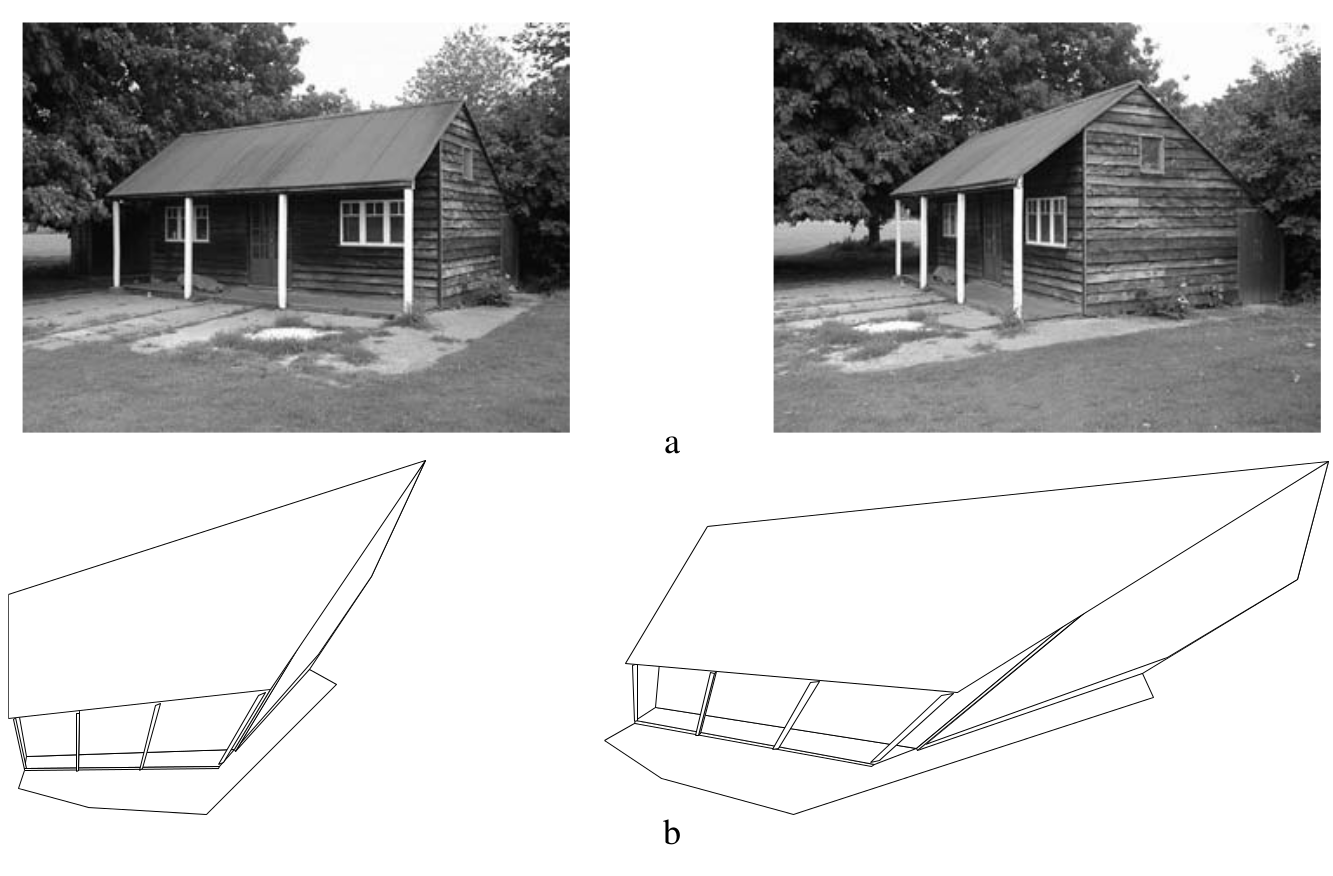
\includegraphics[width=1.0\textwidth]{images/projectivereconstruction.png}
\caption[Reconstrucci\'{o}n proyectiva]%
{\textbf{(a)} Par de im\'{a}genes originales. \textbf{(b)} Dos vistas de una reconstrucci\'{o}n proyectiva de la escena. La reconstrucci\'{o}n no requiere informaci\'{o}n acerca de las matrices de la c\'{a}mara o de la geometr\'{i}a de la escena. La matriz fundamental \textit{F} se calcula a partir de correspondencia de puntos entre el par de im\'{a}genes. Las matrices de la c\'{a}mara se obtienen a partir de \textit{F} y finalmente, los puntos tridimensionales son calculados por medio de triangulaci\'{o}n a partir de las correspondencias. Imagen tomada del libro \textit{Multiple View Geometry} de Richard Hartley y Andrew Zisserman \copyright.}
\label{fig:ProjectiveReconstruction}
\end{figure}


Sin embargo, para la t\'{e}cnica propuesta se busca una reconstrucci\'{o}n m\'{e}trica por lo que para el proceso de estimaci\'{o}n de la profundidad es necesario utilizar la matriz esencial \textit{E} en lugar de la matriz fundamental \textit{F}. En la figura ~\ref{fig:MetricReconstruction} se muestra un ejemplo de reconstrucci\'{o}n m\'{e}trica.


\begin{figure}[H]
\centering
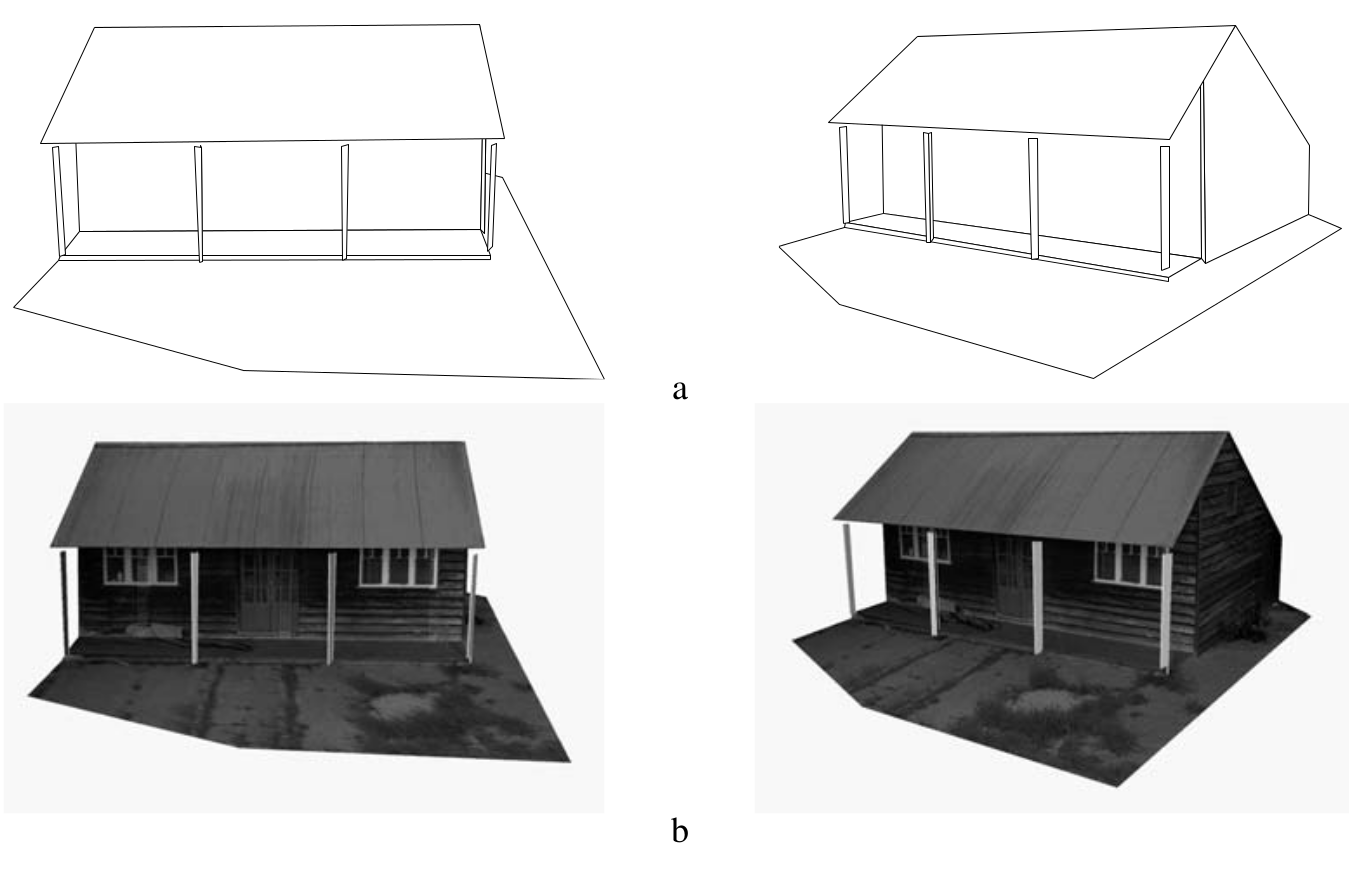
\includegraphics[width=1.0\textwidth]{images/metricreconstruction.png}
\caption[Reconstrucci\'{o}n m\'{e}trica]%
{\textbf{(a)} Dos vistas de la reconstrucci\'{o}n m\'{e}trica. L\'{i}neas que son perpendiculares en la escena son perpendiculares en la reconstrucci\'{o}n y tambi\'{e}n la relaci\'{o}n de aspecto de los lados de la casa es ver\'{i}dico. \textbf{(b)} Dos vistas del modelo reconstruido con textura. Imagen tomada del libro \textit{Multiple View Geometry} de Richard Hartley y Andrew Zisserman \copyright.}
\label{fig:MetricReconstruction}
\end{figure}


Para encontrar la posición de un punto bidimensional en el espacio tridimensional, hay que determinar la posici\'{o}n/orientaci\'{o}n de la c\'{a}mara cuando tom\'{o} la primera imagen (c\'{a}mara P) que contiene a ese punto, luego determinar la posici\'{o}n/orientaci\'{o}n de la c\'{a}mara cuando tom\'{o} la segunda imagen (c\'{a}mara P') de ese mismo punto y finalmente, utilizar el m\'{e}todo lineal de triangulaci\'{o}n seleccionado en la fase anterior. Esto se logra por medio de las ecuaciones $x = PX$ y $x' = P'X$, donde \textit{x} y \textit{x'} son el pareo de puntos bidimensionales y \textit{X} es la posici\'{o}n tridimensional real del punto presentado en ambas c\'{a}maras.

Es posible reescribir las ecuaciones como un sistema lineal que puede resolverse para determinar \textit{X}, lo cual es el objetivo buscado. Ambas ecuaciones se combinan de la forma $AX = 0$, la cual es una ecuaci\'{o}n lineal en \textit{X}. El siguiente planteamiento del sistema de ecuaciones lineales utilizado para la t\'{e}cnica de reconstrucci\'{o}n fue tomado directamente de \cite{Hartley_Zisserman_2003}. Primero, el factor de escala homog\'{e}neo es eliminado con un producto cruzado para obtener tres ecuaciones por cada punto de la imagen, de los cuales dos son linealmente independientes. Por ejemplo, para la primera imagen, $x \times (PX) = 0$ lo cual da:


\vspace{5 mm}
\begin{center}
$x(p^{3T}X) - (p^{1T}X) = 0$ \\
$y(p^{3T}X) - (p^{2T}X) = 0$ \\
$x(p^{2T}X) - y(p^{1T}X) = 0$
\end{center}
\vspace{5 mm}


donde $p^{iT}$ son las filas de la matriz $P$. Estas ecuaciones son lineales en los componentes de \textbf{X}. Una ecuaci\'{o}n de la forma $AX = 0$ puede ser entonces creada con:

\vspace{5 mm}
\begin{center}
$\textbf{\textit{A}} =
\left[ {
\begin{array}{*{20}c}
   xp^{3T} - p^{1T} \\
   yp^{3T} - p^{2T} \\
   x'p'^{3T} - p'^{1T} \\
   y'p'^{3T} - p'^{2T} \\
\end{array} 
} \right]$
\end{center}
\vspace{5 mm}

donde dos ecuaciones han sido incluidas para cada imagen, dando un total de cuatro ecuaciones con cuatro inc\'{o}gnitas homog\'{e}neas. \'{E}ste es un conjunto de ecuaciones redundantes, dado que la soluci\'{o}n es determinada a escala. La descripci\'{o}n completa de la soluci\'{o}n puede encontrarse en \cite{Hartley_Zisserman_2003}. Con la soluci\'{o}n del sistema de ecuaciones anterior es posible obtener una aproximaci\'{o}n de los puntos tridimensionales a partir de dos puntos bidimensionales. 

El proceso final para completar la estructura tridimensional del objeto es iterar sobre cada par de puntos obtenidos, realizar la triangulaci\'{o}n y almacenar el punto tridimensional en una lista para su posterior visualizaci\'{o}n. A continuaci\'{o}n, se muestran diferentes resultados obtenidos con la t\'{e}cnica r\'{a}pida de reconstrucci\'{o}n propuesta.


\begin{figure}[H]
\centering
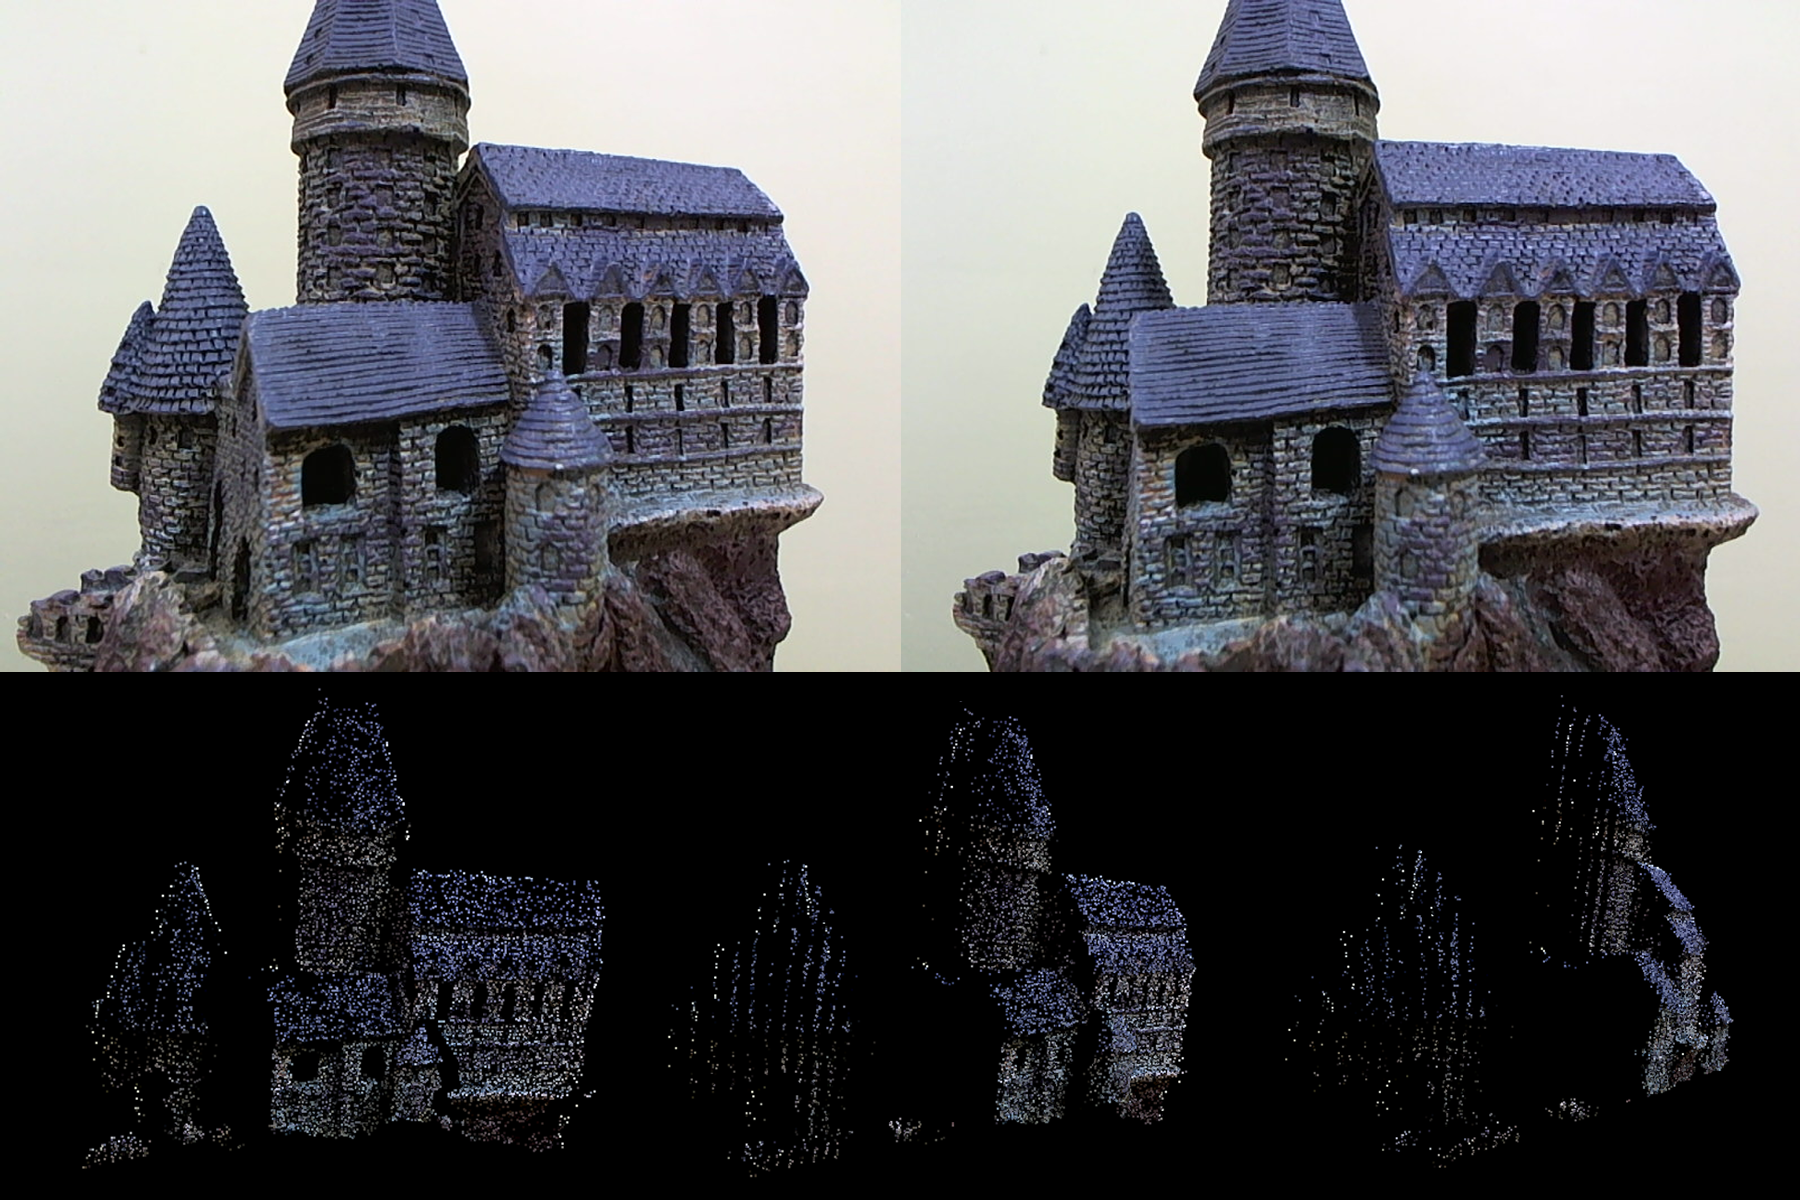
\includegraphics[width=1.0\textwidth]{images/reconstruction1.png}
\caption[Reconstrucci\'{o}n de un costado del castillo]%
{Reconstrucci\'{o}n tridimensional de un costado del casillo utilizando un par de im\'{a}genes estereosc\'{o}picas. N\'{o}tese la densidad de la reconstrucci\'{o}n as\'{i} como la precisi\'{o}n entre las diferentes profundidades del techo y de las torres. Im\'{a}genes generadas con la t\'{e}cnica de reconstrucción propuesta.}
\label{fig:Reconstruction1}
\end{figure}

En la figura ~\ref{fig:Reconstruction1} se muestra la reconstrucci\'{o}n de un costado del castillo a partir de un par de im\'{a}genes estereosc\'{o}picas utilizando la t\'{e}cnica propuesta. N\'{o}tese la densidad de la reconstrucci\'{o}n as\'{i} como la precisi\'{o}n entre las diferentes profundidades del techo y de las torres.


\begin{figure}[H]
\centering
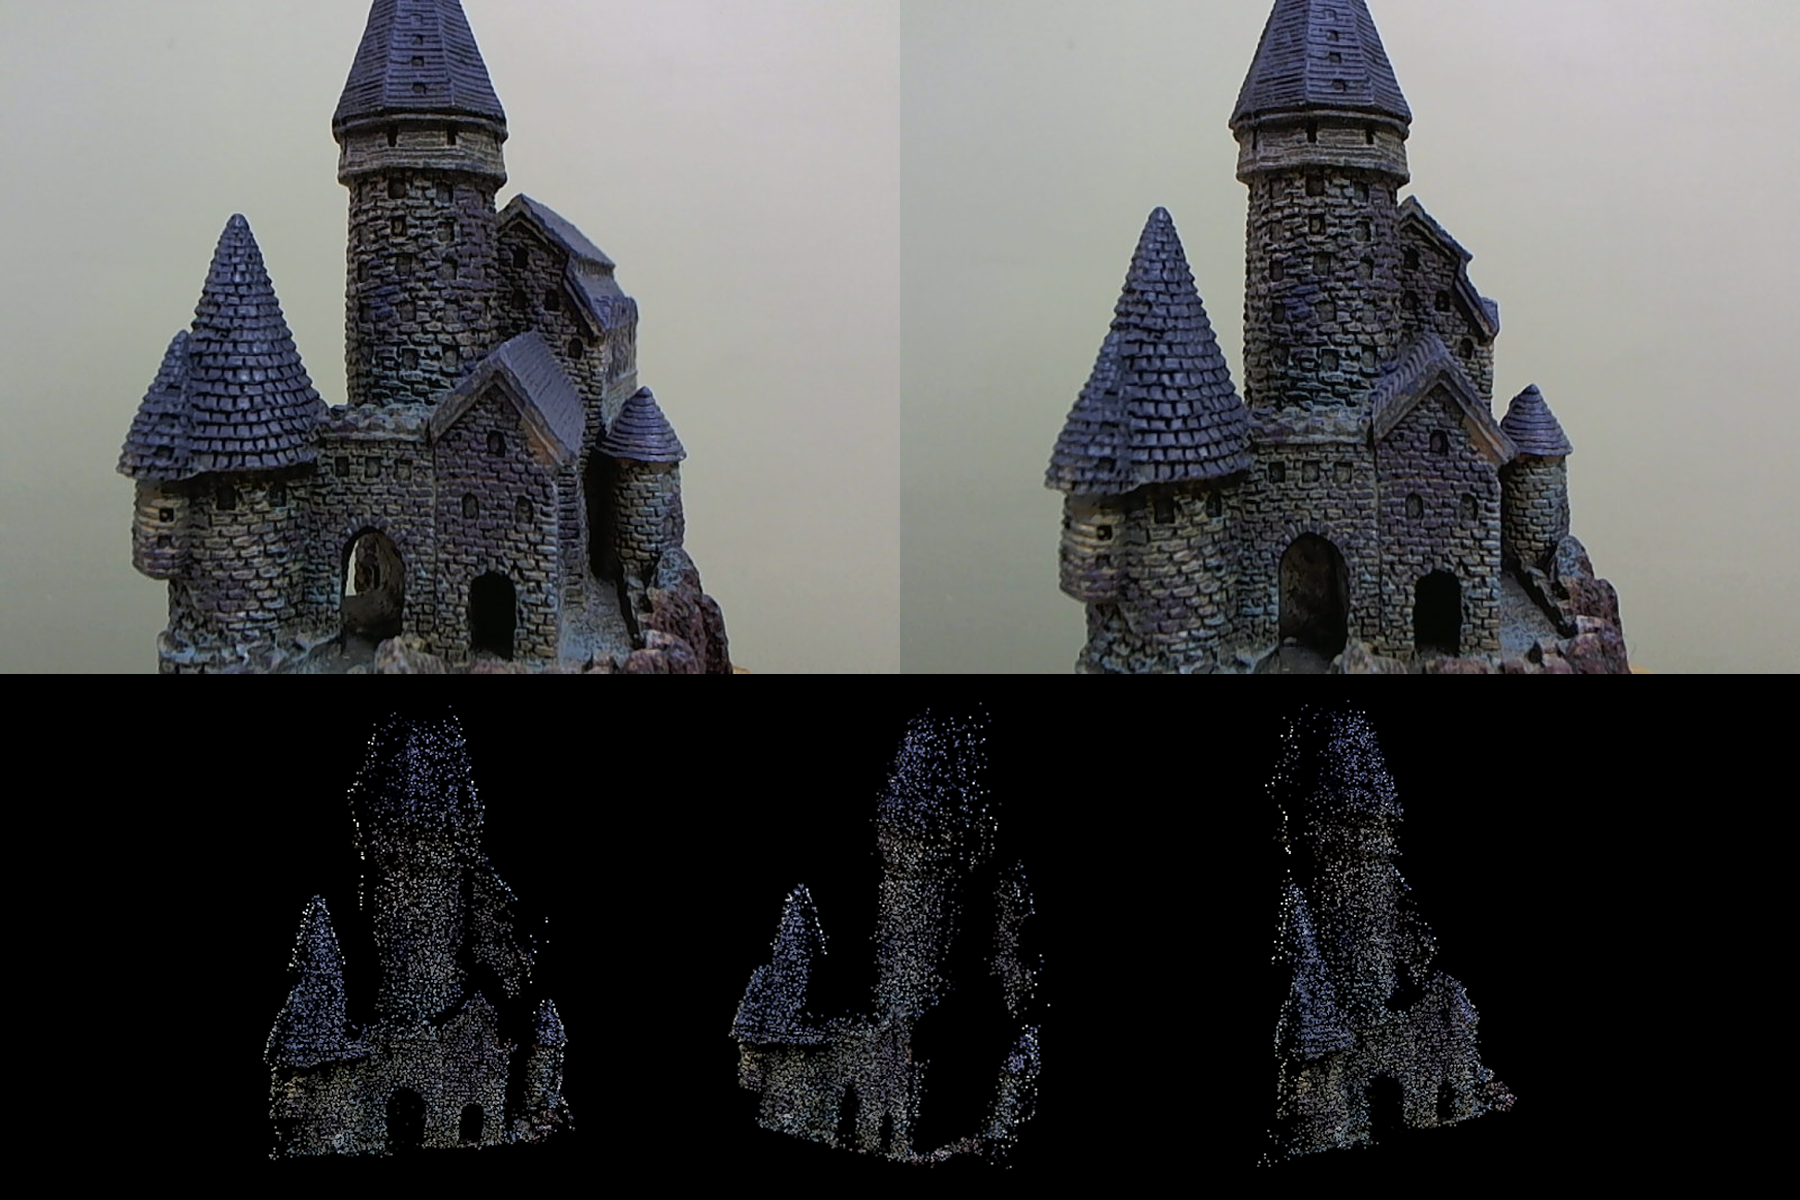
\includegraphics[width=1.0\textwidth]{images/reconstruction2.png}
\caption[Reconstrucci\'{o}n de la fachada del castillo]%
{Reconstrucci\'{o}n tridimensional de la fachada del casillo utilizando un par de im\'{a}genes estereosc\'{o}picas. Nuevamente, n\'{o}tese la precisi\'{o}n de la profundidad entre una torre y la otra. Im\'{a}genes generadas con la t\'{e}cnica de reconstrucción propuesta.}
\label{fig:Reconstruction2}
\end{figure}


En la figura ~\ref{fig:Reconstruction2} se muestra la reconstrucci\'{o}n de la fachada del castillo a partir de un par de im\'{a}genes estereosc\'{o}picas. Nuevamente, n\'{o}tese la precisi\'{o}n de la profundidad reconstruida entre una torre y la otra.


\begin{figure}[H]
\centering
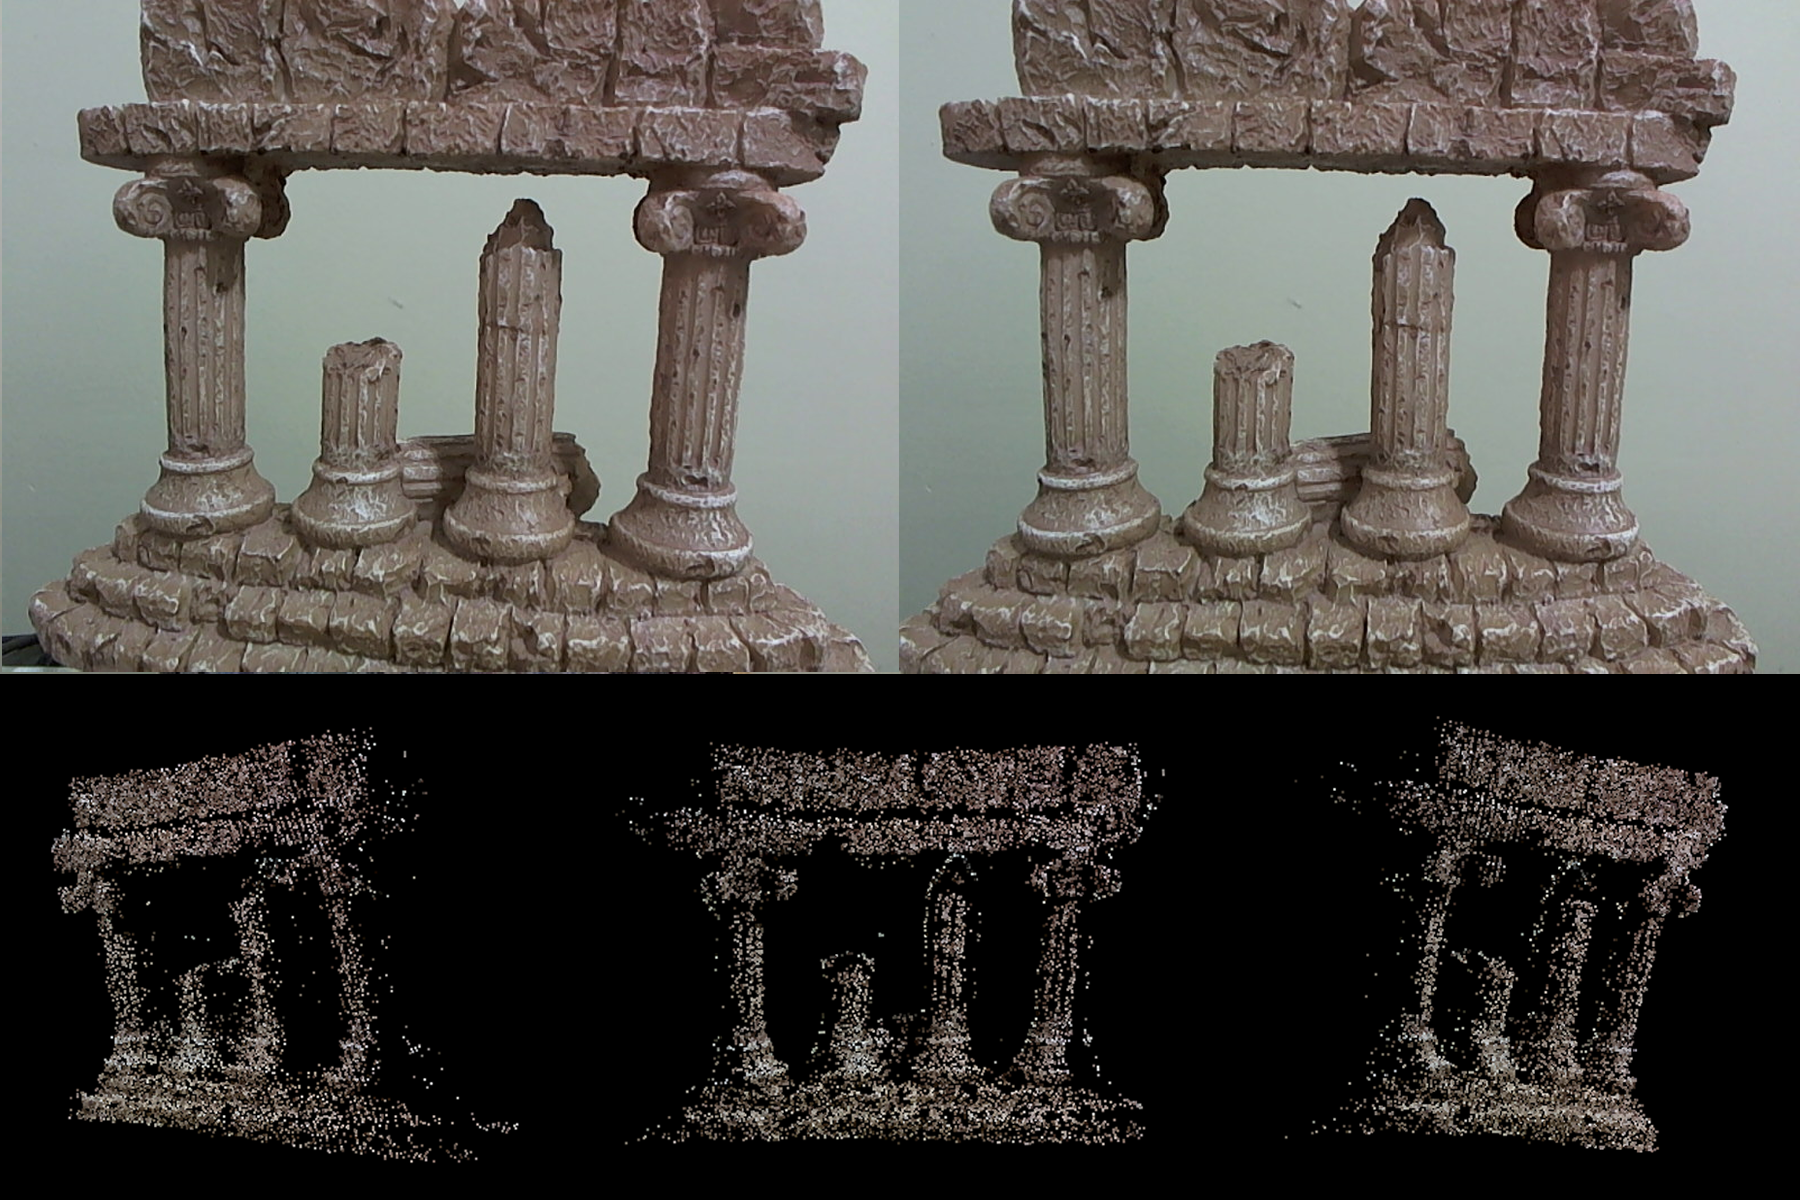
\includegraphics[width=0.9\textwidth]{images/reconstruction3.png}
\caption[Reconstrucci\'{o}n de las columnas Griegas]%
{Reconstrucci\'{o}n tridimensional de las columnas Griegas utilizando un par de im\'{a}genes estereosc\'{o}picas. Por su particular forma, la reconstrucci\'{o}n de este objeto es m\'{a}s compleja que el castillo pero de igual manera se logr\'{o} obtener resultados satisfactorios. Im\'{a}genes generadas con la t\'{e}cnica de reconstrucción propuesta.}
\label{fig:Reconstruction3}
\end{figure}


Finalmente, en la figura ~\ref{fig:Reconstruction3} se muestra la reconstrucci\'{o}n de unas columnas Griegas. A pesar de su particular forma y de la diferencia estructural con respecto al castillo, se logr\'{o} obtener resultados satisfactorios. Cabe destacar que en todos los casos presentados el proceso completo de reconstrucci\'{o}n tom\'{o} no m\'{a}s que unos cuantos segundos.


\section{Reconstrucci\'{o}n con m\'{a}s de dos vistas}
Es posible obtener una reconstrucci\'{o}n a\'{u}n m\'{a}s densa utilizando vistas adicionales del objeto. Para lograr esto se implement\'{o} un m\'{e}todo simple basado en una variante lineal del problema de \textit{Perspective-n-Point} o \textit{PnP} que permite la recuperaci\'{o}n de informaci\'{o}n tridimensional adicional a partir de nuevas vistas del objeto. A la variante se le conoce como \textit{Efficient Perspective-n-Point} o \textit{EPnP}\cite{F_Moreno_V_Lepetit}.

El algoritmo de \textit{PnP} pretende resolver el problema de c\'{o}mo determinar la posici\'{o}n y orientaci\'{o}n de la c\'{a}mara dados sus par\'{a}metros intr\'{i}nsecos m\'{a}s un conjunto de \textit{n} correspondencias entre puntos tridimensionales y sus proyecciones bidimensionales \cite{F_Moreno_V_Lepetit}. Esto significa que con \textit{PnP} es posible estimar la posici\'{o}n de subsecuentes c\'{a}maras (vistas) del objeto a reconstruir utilizando la informaci\'{o}n obtenida (matrices y pareos) en las fases anteriores.

Para incorporar nuevas vistas a la reconstrucci\'{o}n, es necesario encontrar la posici\'{o}n de cada nueva c\'{a}mara utilizando como base la estructura inicial obtenida en la triangulaci\'{o}n de la fase anterior. Para esto se procede a buscar mapeos entre los puntos bidimensionales encontrados en la nueva vista y los puntos tridimensionales ya obtenidos. El objetivo del mapeo es obtener una lista de puntos bidimensionales y otra de puntos tridimensionales en la cual el punto bidimensional \textit{i} corresponde al punto tridimensional \textit{i} dado que es un requisito del algoritmo \textit{EPnP}. Finalmente, se utiliza la matriz \textit{K} en conjunto con los mapeos como entrada del algoritmo de \textit{EPnP} para obtener la posici\'{o}n de la c\'{a}mara (\textit{P1}) de esa nueva vista.

Obtenida la matriz \textit{P1} de la nueva c\'{a}mara, se procede a triangular los puntos de la nueva vista como se realiz\'{o} en la etapa anterior. Finalmente, se almacenan los puntos tridimensionales resultantes en la lista global de puntos 3D y se procede a repetir el proceso para las vistas restantes.

En la figura ~\ref{fig:Castle234} se muestra un ejemplo de reconstrucci\'{o}n con 2, 3 y 4 vistas para el castillo. Cuando la reconstrucci\'{o}n se limita a 2 o 3 vistas la t\'{e}cnica propuesta genera resultados muy satisfactorios como se puede observar en la figura.


\begin{figure}[H]
\centering
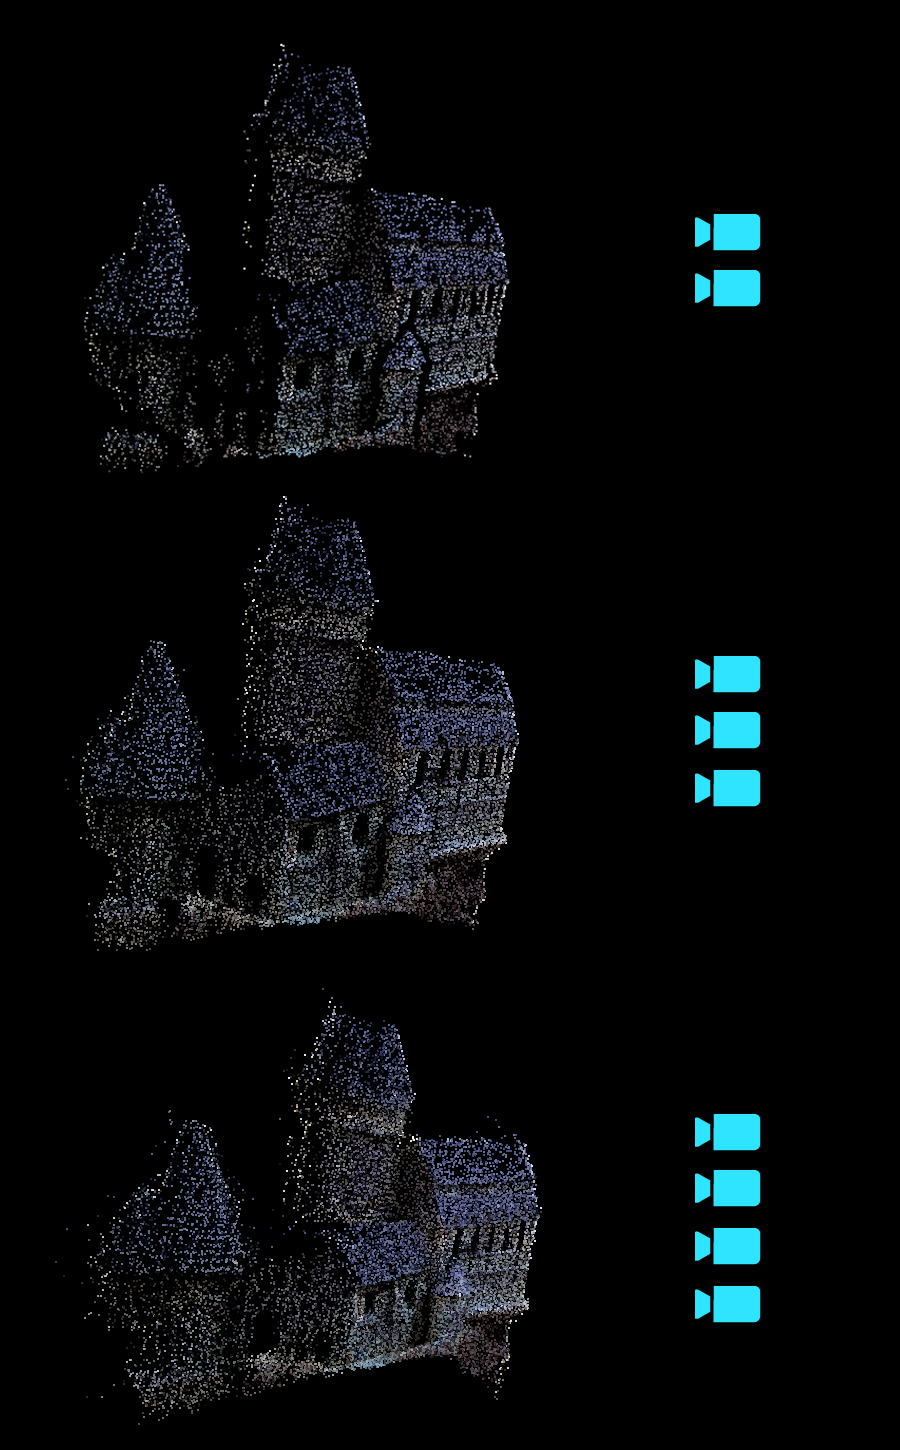
\includegraphics[width=0.8\textwidth]{images/castle234.png}
\caption[Reconstrucci\'{o}n del casillo con 2, 3 y 4 vistas]%
{Reconstrucci\'{o}n tridimensional del castillo con 2, 3 y 4 vistas. La necesidad de una etapa de refinamiento se nota m\'{a}s claramente en la reconstrucci\'{o}n con cuatro vistas. Im\'{a}genes generadas con la t\'{e}cnica de reconstrucción propuesta.}
\label{fig:Castle234}
\end{figure}


Sin embargo, cuando se incrementa a 4 o m\'{a}s vistas los nuevos puntos triangulados no se encuentran completamente alineados con los triangulados previamente. Esto se debe a que cada reconstrucci\'{o}n obtenida a partir del par de im\'{a}genes estereosc\'{o}picas posee su propia escala la cual es totalmente independiente de las escalas de las siguientes reconstrucciones. Una forma de atacar este problema es introducir una etapa de refinamiento y registro al final de cada reconstrucci\'{o}n pero dichas etapas no forman parte de esta tesis.

\begin{figure}[H]
\centering
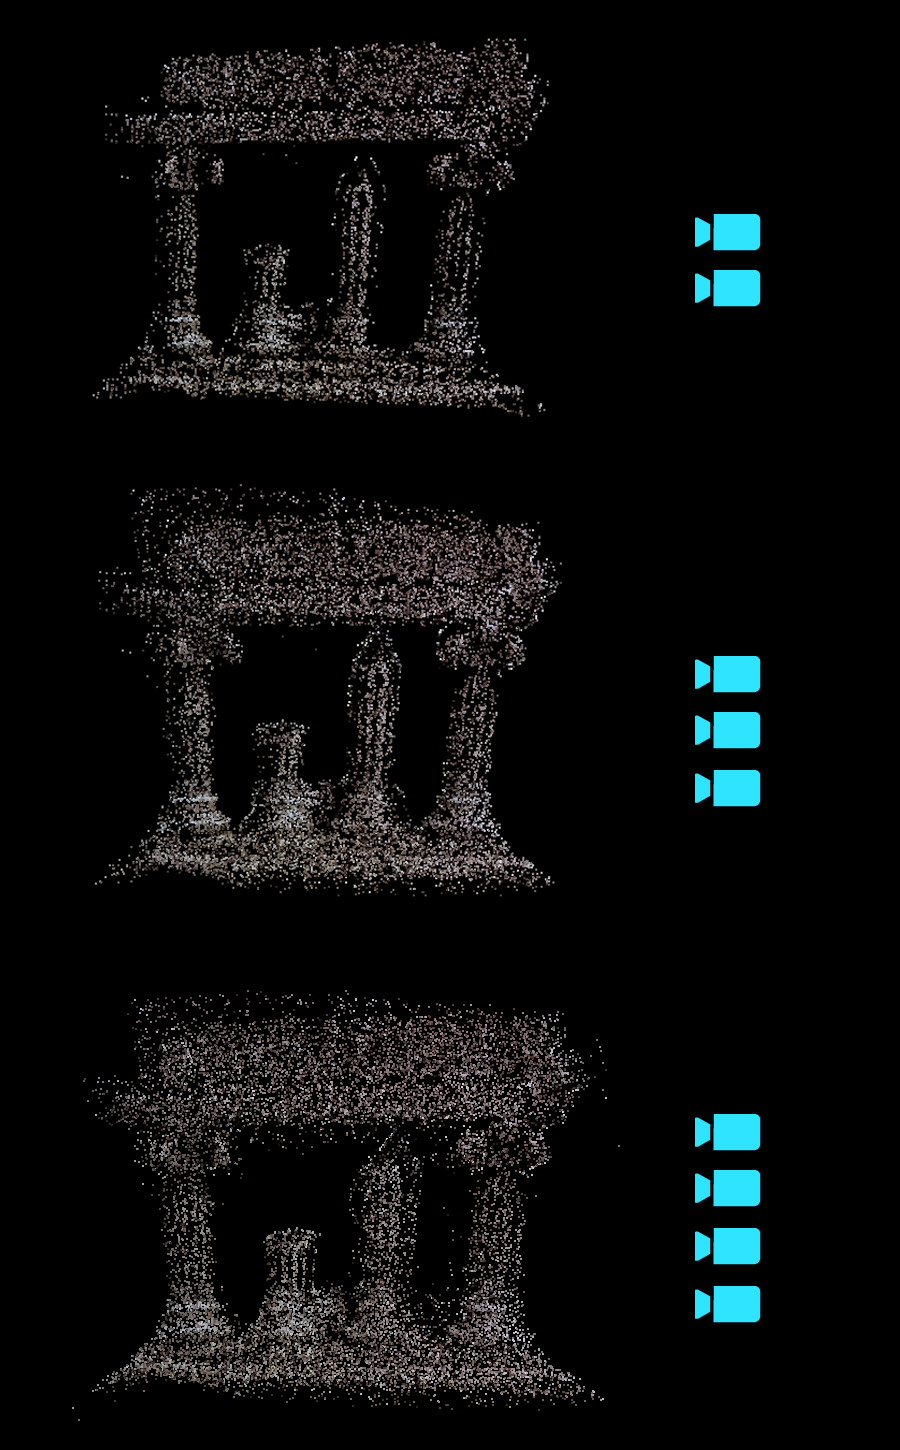
\includegraphics[width=0.8\textwidth]{images/greek234.png}
\caption[Reconstrucci\'{o}n de las columnas Griegas con 2, 3 y 4 vistas]%
{Reconstrucci\'{o}n tridimensional las columnas Griegas con 2, 3 y 4 vistas. Nuevamente, se nota la necesidad de una etapa de refinamiento en este caso a partir de la reconstrucci\'{o}n con tres vistas. Im\'{a}genes generadas con la t\'{e}cnica de reconstrucción propuesta.}
\label{fig:Greek234}
\end{figure}


En la figura ~\ref{fig:Greek234} se muestra otro ejemplo de reconstrucci\'{o}n con 2, 3 y 4 vistas para las columnas Griegas. Nuevamente se puede observar que con 2 vistas la reconstrucci\'{o}n es bastante satisfactoria pero en este caso a partir de la vista 3, la reconstrucci\'{o}n se ve afectada por la falta de las etapas de refinamiento y registro.

Cabe destacar que para lograr la reconstrucci\'{o}n completa de un objeto es necesaria la incorporaci\'{o}n de etapas de refinamiento y registro, sin embargo ambas etapas est\'{a}n fuera de los alcances de esta tesis y se dejar\'{a}n para trabajo futuro.


%@TODO hablar de reconstrucción utilizando multiples vistas, del error de retroproyección y de que bundle adjusment refinaria aun mas la reconstruccion. Hablar de que no se hizo registracion por lo que no hay reconstruccion completa.

%@TODO resumen del capitulo
